\newpage

\section{Caso de estudio 2, $R_i=100[k\Omega]$}

\subsection{Diseño de la etapa.}
\onehalfspacing
En este caso se deben cumplir los mismos requisitos descriptos en el inciso anterior
\paragraph{}
A partir de dichas especificaciones se obtiene:
\begin{equation}
    \nonumber
    R_i=50[\Omega] \longrightarrow Z_{i1,2} \geq 10R_i = 1[M\Omega]
\end{equation}
donde $Z_{i1,2} = R$.
\paragraph{}
Como el valor obtenido es el límite máximo admitido se toma $R=1[M\Omega]$. Si $A_{v1,2}(0)=30$
\begin{equation}
    \nonumber
    \frac{R_f}{R}=30 \longrightarrow R_f=30[M\Omega]
\end{equation}
\paragraph{}
En este caso $R_f >> 10[M\Omega]$ razón por la cual se hace uso de una red $T$ para cumplir con las especificaciones solicitadas.

\subsubsection{Red T.}
\onehalfspacing
Para el diseño de la \textit{red T} se debe tener en cuenta la relación entre $V_O$ y la corriente de alimentación $i_f$ que pasa por la resistencia $R_1$.
\paragraph{}
Suponiendo la entrada inversora a masa,
\begin{align}
    \nonumber
    i_f &= \frac{V_O}{R_2 + R_1||R_3}\cdot R_1||R_3 \cdot \frac{1}{R_1} \\
    \nonumber
    i_f &= \frac{R_3}{R_2\cdot R_1 + R_2\cdot R_3 + R_3\cdot R_1} \cdot V_O \\
    \nonumber
    \frac{V_O}{i_f} &= \frac{R_2 \cdot R_1}{R_3} + R_2 + R_1
\end{align}

\paragraph{}
Si $\frac{V_O}{i_f}=R_f$,
\begin{center}
    \boxed{R_f = \frac{R_2 \cdot R_1}{R_3} + R_2 + R_1}
\end{center}

\paragraph{}
Tomando  $R_1 = 100[k\Omega]$ y $R_2 = 220[k\Omega]$ con $R_f=30[M\Omega]$,
\begin{center}
    \boxed{R_3 = 741[\Omega]}
\end{center}

\paragraph{}
De esta manera se logran satisfacer todas las especificaciones.

\subsection{Cálculo de errores.}
\onehalfspacing
Con la incorporación de la red T la ganancia de lazo cambia a:
%\begin{equation}
%    \nonumber
%    T = - \frac{1}{2}\cdot \frac{A_d \cdot R \cdot R_3}{\left( 
%R_1 + \frac{R}{2} \right) \cdot \left( R_2 + R_3 \right) + R_2\cdot R_3}
%\end{equation}

\begin{equation}
    \nonumber
    T = - \frac{1}{2}\cdot \frac{A_d \cdot R \cdot R_3}{\left( 
R_1 + \frac{R}{2} \right) \cdot \left( R_2 + R_3 \right)}
\end{equation}

\subsubsection{Errores en DC.}
\onehalfspacing
\begin{equation}
    \nonumber
    \Delta V_{O}(v_{os}) = 2 \cdot \left( \frac{\left( 
R_1 + \frac{R}{2} \right) \cdot \left( R_2 + R_3 \right)}{R \cdot R_3} \right) \cdot v_{os} = 357,5v_{os} = 357,5\cdot 2[mV]  = 715[mV]
\end{equation}
\begin{equation}
    \nonumber
    \Delta V_{O}(I_{os}) = -R_f\cdot I_p^{-} = 30[M\Omega]\cdot I_p^{-} = 30[M\Omega]\cdot 45[\mu A]  = 1.350[V]
\end{equation}
\begin{equation}
    \nonumber
    \Delta V_{O}(A_d<\infty) = \frac{FS}{T_O} = \frac{10[V]}{280} = 35,7[mV]
\end{equation}
\begin{equation}
    \nonumber
    \Delta V_{O}(RRMC<\infty) = 0[V]
\end{equation}

\paragraph{}
El error total resulta: 

\begin{center}
    \boxed{\Delta V_{o} = 2,1[V]}
\end{center}

\subsubsection{Errores en AC.}
\onehalfspacing
\textbf{Ancho de banda de plena potencia.} 
\paragraph{}
\begin{equation}
    \nonumber
    f_{HP} = \frac{SR}{2\pi \cdot V_{pp}} =  \frac{0.5\left[ \frac{V}{uS} \right]}{2\pi \cdot 10[V]} = 8[kHz]
\end{equation}

\paragraph{}
\textbf{Ancho de banda de pequeña señal.} 
\paragraph{}
\begin{equation}
    \nonumber
    f_{HP} = k\cdot f_T = \frac{f_T}{A_{vfi}} = 33,3[kHz]
\end{equation}

\paragraph{}
Debido a que el amplificador utilizado en la simulación es de segundo órden, es decir tiene un polo que no permite que que el ancho de banda llegue a $1[MHz]$, sino que provoca la caída de $3dB$ en $2.7[kHz]$ es necesario recalcular para los $2.7[kHz]$:

\begin{equation}
    \centering
    \nonumber
    f_h = 0.9[kHz]
\end{equation}

\newpage

\textbf{Error vectorial.} 
\paragraph{}
\begin{figure}[h!]
    \centering
    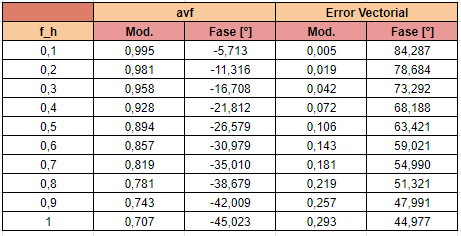
\includegraphics{figuras/lab_2_tabla_ev2.PNG}
    \caption{Error vectorial}
    \label{fig:enter-label}
\end{figure}
  
\subsection{Simulaciones.}
\onehalfspacing
A continuación se adjuntan las simulaciones para el circuito bajo estudio

\begin{figure}[h!]
    \centering
    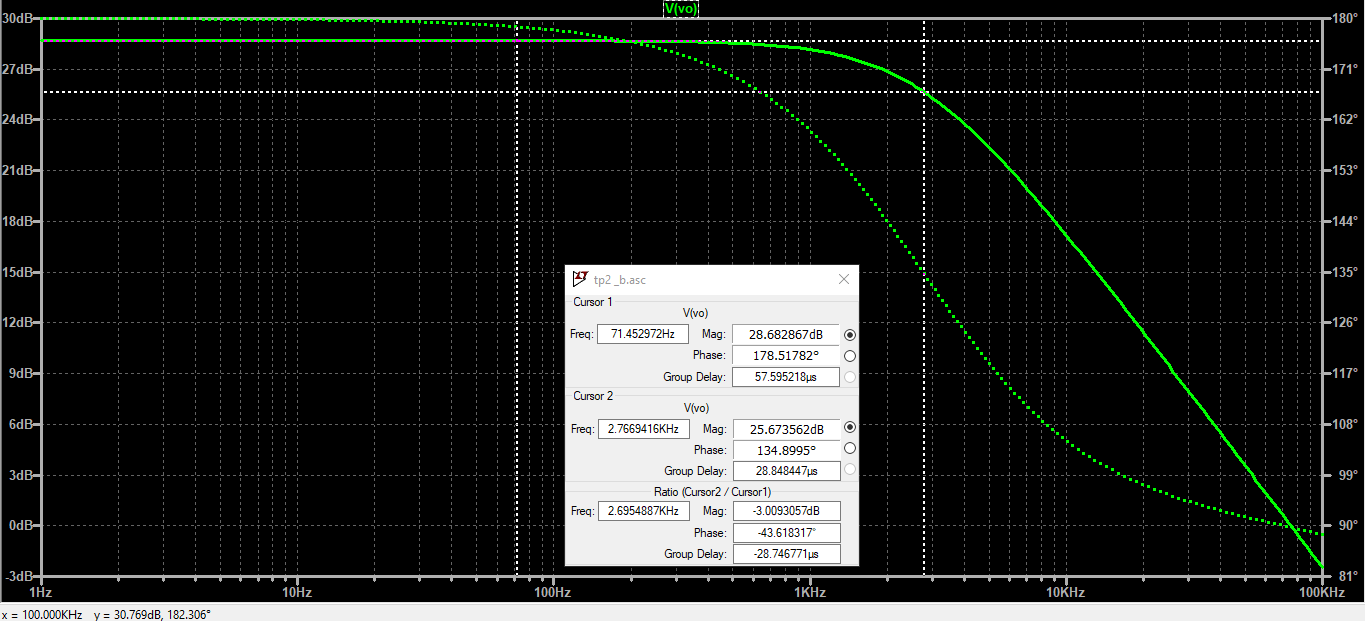
\includegraphics[scale=0.4]{figuras/simulacion2/bode_barrido_hasta100k.png}
    \caption{Barrido en frecuencia, hasta $100kHz$}
    \label{fig:enter-label}
\end{figure}

\begin{figure}[h!]
    \centering
    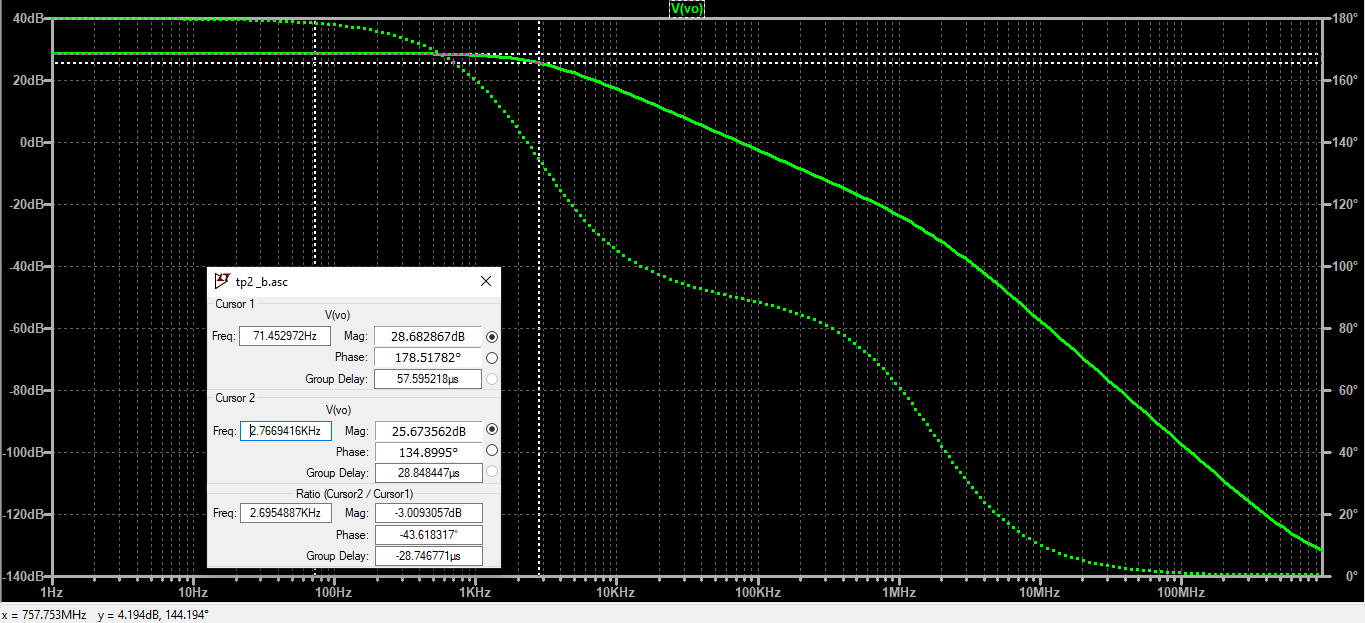
\includegraphics[scale=0.4]{figuras/simulacion2/bode_barrido_hasta1G.png}
    \caption{Barrido en frecuencia, hasta $1GHz$}
    \label{fig:enter-label}
\end{figure}

\begin{figure}[h!]
    \centering
    
\includegraphics[scale=0.4]{figuras/simulacion2/Vo_Ios_CC.png}
    \caption{Vout(Vos)}
    \label{fig:enter-label}
\end{figure}